%%
%% This is file `sample-sigconf.tex',
%% generated with the docstrip utility.
%%
%% The original source files were:
%%
%% samples.dtx  (with options: `sigconf')
%% 
%% IMPORTANT NOTICE:
%% 
%% For the copyright see the source file.
%% 
%% Any modified versions of this file must be renamed
%% with new filenames distinct from sample-sigconf.tex.
%% 
%% For distribution of the original source see the terms
%% for copying and modification in the file samples.dtx.
%% 
%% This generated file may be distributed as long as the
%% original source files, as listed above, are part of the
%% same distribution. (The sources need not necessarily be
%% in the same archive or directory.)
%%
%% The first command in your LaTeX source must be the \documentclass command.
\documentclass[sigconf]{acmart}
%% NOTE that a single column version may be required for 
%% submission and peer review. This can be done by changing
%% the \doucmentclass[...]{acmart} in this template to 
%% \documentclass[manuscript,screen]{acmart}
%% 
%% To ensure 100% compatibility, please check the white list of
%% approved LaTeX packages to be used with the Master Article Template at
%% https://www.acm.org/publications/taps/whitelist-of-latex-packages 
%% before creating your document. The white list page provides 
%% information on how to submit additional LaTeX packages for 
%% review and adoption.
%% Fonts used in the template cannot be substituted; margin 
%% adjustments are not allowed.
%%
%%


\usepackage{colortbl}
\usepackage{xcolor}
\usepackage{multirow}

%% Rights management information.  This information is sent to you
%% when you complete the rights form.  These commands have SAMPLE
%% values in them; it is your responsibility as an author to replace
%% the commands and values with those provided to you when you
%% complete the rights form.
\setcopyright{acmcopyright}
\copyrightyear{2018}
\acmYear{2018}
\acmDOI{10.1145/1122445.1122456}

%% These commands are for a PROCEEDINGS abstract or paper.
\acmConference[Woodstock '18]{Woodstock '18: ACM Symposium on Neural
  Gaze Detection}{June 03--05, 2018}{Woodstock, NY}
\acmBooktitle{Woodstock '18: ACM Symposium on Neural Gaze Detection,
  June 03--05, 2018, Woodstock, NY}
\acmPrice{15.00}
\acmISBN{978-1-4503-XXXX-X/18/06}


%%
%% Submission ID.
%% Use this when submitting an article to a sponsored event. You'll
%% receive a unique submission ID from the organizers
%% of the event, and this ID should be used as the parameter to this command.
%%\acmSubmissionID{123-A56-BU3}

%%
%% The majority of ACM publications use numbered citations and
%% references.  The command \citestyle{authoryear} switches to the
%% "author year" style.
%%
%% If you are preparing content for an event
%% sponsored by ACM SIGGRAPH, you must use the "author year" style of
%% citations and references.
%% Uncommenting
%% the next command will enable that style.
%%\citestyle{acmauthoryear}

%%
%% end of the preamble, start of the body of the document source.
\begin{document}

%%
%% The "title" command has an optional parameter,
%% allowing the author to define a "short title" to be used in page headers.
\title{GLL-based Context-Free Path Querying for Neo4j}

%%
%% The "author" command and its associated commands are used to define
%% the authors and their affiliations.
%% Of note is the shared affiliation of the first two authors, and the
%% "authornote" and "authornotemark" commands
%% used to denote shared contribution to the research.
\author{Vlada Pogozhelskaya}
\affiliation{%
  \institution{Saint Petersburg State University}
  \streetaddress{7/9 Universitetskaya nab.}
  \city{St. Petersburg}
  \country{Russia}
  \postcode{199034}
}
\affiliation{
		\institution{JetBrains Research}
		\streetaddress{Primorskiy prospekt 68-70, Building 1}
		\city{St. Petersburg}
		\country{Russia}
		\postcode{199034}
	}
\email{pogozhelskaya@gmail.com}
%\orcid{1234-5678-9012}


\author{Anna Vlasova}
\affiliation{
		\institution{JetBrains Research}
		\streetaddress{Primorskiy prospekt 68-70, Building 1}
		\city{St. Petersburg}
		\country{Russia}
		\postcode{199034}
	}
\email{anna.vlasova@jetbrains.com}
%\orcid{1234-5678-9012}

\author{Semyon Grigorev}
\affiliation{
		\institution{Saint Petersburg State University}
		\streetaddress{7/9 Universitetskaya nab.}
		\city{St. Petersburg}
		\country{Russia}
		\postcode{199034}
	}
	\affiliation{
		\institution{JetBrains Research}
		\streetaddress{Primorskiy prospekt 68-70, Building 1}
		\city{St. Petersburg}
		\country{Russia}
		\postcode{199034}
	}
\email{s.v.grigoriev@spbu.ru}
\email{semyon.grigorev@jetbrains.com}
\orcid{0000-0002-7966-0698}


%%
%% By default, the full list of authors will be used in the page
%% headers. Often, this list is too long, and will overlap
%% other information printed in the page headers. This command allows
%% the author to define a more concise list
%% of authors' names for this purpose.
\renewcommand{\shortauthors}{Pogozhelskaya, Vlasova, Grigorev.}

%%
%% The abstract is a short summary of the work to be presented in the
%% article.
\begin{abstract}
  We show that a fast GLL parsing algorithm provides \textit{context-free path querying} for Neo4j graph database with reasonable performance. The proposed solution solves both the \textit{reachability} and the \textit{all paths} problems for the \textit{all pairs} and the \textit{multiple sources} cases. The evaluation on real-world graphs demonstrates that our solution is more than 25 times faster than the previous solution for Neo4j and is comparable, in some cases,  with the linear algebra based solution for RedisGraph.
\end{abstract}

%%
%% The code below is generated by the tool at http://dl.acm.org/ccs.cfm.
%% Please copy and paste the code instead of the example below.
%%
\begin{CCSXML}
		<ccs2012>
		<concept>
			<concept_id>10002951.10002952.10003197.10010825</concept_id>
			<concept_desc>Information systems~Query languages for non-relational engines</concept_desc>
			<concept_significance>500</concept_significance>
		</concept>
		<concept>
			<concept_id>10003752.10003766.10003771</concept_id>
			<concept_desc>Theory of computation~Grammars and context-free languages</concept_desc>
			<concept_significance>500</concept_significance>
		</concept>
		<concept>
			<concept_id>10002950.10003624.10003633.10003640</concept_id>
			<concept_desc>Mathematics of computing~Paths and connectivity problems</concept_desc>
			<concept_significance>300</concept_significance>
		</concept>
		<concept>
			<concept_id>10002951.10002952.10002953.10010146</concept_id>
			<concept_desc>Information systems~Graph-based database models</concept_desc>
			<concept_significance>500</concept_significance>
		</concept>
		</ccs2012>
\end{CCSXML}

    \ccsdesc[500]{Information systems~Graph-based database models}
	\ccsdesc[500]{Information systems~Query languages for non-relational engines}
	\ccsdesc[500]{Theory of computation~Grammars and context-free languages}
    \ccsdesc[300]{Mathematics of computing~Paths and connectivity problems}

%%
%% Keywords. The author(s) should pick words that accurately describe
%% the work being presented. Separate the keywords with commas.
\keywords{Graph database, context-free path querying, CFPQ, reachability problem, all paths problem, generalized LL, GLL}

%%
%% This command processes the author and affiliation and title
%% information and builds the first part of the formatted document.
\maketitle

\section{Introduction}

Scalable high-performance graph analysis is an actual challenge.
There is a big number of ways to attack this challenge~\cite{Coimbra2021} and the first promising idea is to utilize general-purpose graphic processing units (GPGPU-s).
Such existing solutions, as CuSha~\cite{10.1145/2600212.2600227} and Gunrock~\cite{7967137} show that utilization of GPUs can improve the performance of graph analysis, moreover it is shown that solutions may be scaled to multi-GPU systems.
But low flexibility and high complexity of API are problems of these solutions.

The second promising thing which provides a user-friendly API for high-performance graph analysis algorithms creation is a GraphBLAS API~\cite{7761646} which provides linear algebra based building blocks to create graph analysis algorithms.
The idea of GraphBLAS is based on is a well-known fact that linear algebra operations can be efficiently implemented on parallel hardware.
Along with this, a graph can be natively represented using matrices: adjacency matrix, incidence matrix, etc.
While reference CPU-based implementation of GraphBLAS, SuiteSparse:GraphBLAS~\cite{10.1145/3322125}, demonstrates good performance in real-world tasks, GPU-based implementation is challenging.

One of the challenges in this way is that real data are often sparse, thus underlying matrices and vectors are also sparse, and, as a result, classical dense data structures and respective algorithms are inefficient. 
So, it is necessary to use advanced data structures and procedures to implement sparse linear algebra, but the efficient implementation of them on GPU is hard due to the irregularity of workload and data access patterns.
Though such well-known libraries as cuSparse show that sparse linear algebra operations can be efficiently implemented for GPGPU-s, it is not so trivial to implement GraphBLAS on GPGPU. 
First of all, it requires \textit{generic} sparse linear algebra, thus it is impossible just to reuse existing libraries which are almost all specified for operations over floats.
The second problem is specific optimizations, such as maskings fusion, which can not be natively implemented on top of existing kernels.
Nevertheless, there is a number of implementations of GraphBLAS on GPGPU, such as GraphBLAST:~\cite{yang2019graphblast}, GBTL~\cite{7529957}, which show that GPGPUs utilization can improve the performance of GraphBLAS-based graph analysis solutions.
But these solutions are not portable because they are based on Nvidia Cuda stack.
Moreover, the scalability problem is not solved: all these solutions support only single-GPU, not multi-GPU computations.

To provide portable GPU implementation of GraphBLAS API we developed a \textit{SPLA} library (sources are published on GitHub: \url{https://github.com/JetBrains-Research/spla}).
This library utilizes OpenCL for GPGPU computing to be portable across devices of different vendors.
Moreover, it is initially designed to utilize multiple GPGPUs to be scalable.
To sum up, the contribution of this work is the following.
\begin{itemize}
    \item Design of portable GPU GraphBLAS implementation proposed. The design involves the utilization of multipole GPUS. Additionally, the proposed design is aimed to simplify library tuning and wrappers for different high-level platforms and languages creation. 
    \item Subset of GraphBLAS API, including such operations as masking, matrix-matrix multiplication, matrix-matrix e-wise addition, is implemented. The current implementation is limited by COO and CSR matrix representation format and uses basic algorithms for some operations, but work in progress and more data formats will be supported and advanced algorithms will be implemented in the future.
    \item Preliminary evaluation on such algorithms as breadth-first search (BFS) and triangles counting (TC), and real-world graphs shows portability across different vendors and promising performance: for some problems Spla is comparable with GraphBLAST. Surprisingly, for some problems, the proposed solution on embedded Intel graphic card shows better performance than SuiteSparse:GraphBLAS on the same CPU. At the same time, the evaluation shows that further optimization is required.
\end{itemize} 
\section{Preliminaries}

We introduce !!!!

\subsection{Context-Free Path Querying}

Graph, grammar, etc.

Let $i\pi j$ denote a unique path between nodes $i$ and $j$ of the graph and $l(\pi)$ denotes a unique string which is obtained from the concatenation of edge labels along the path $\pi$.
For a context-free grammar $G = (\Sigma, N, P, S)$ and directed labelled graph $D = (Q, \Sigma, \delta)$, a triple $(A, i, j)$ is \textit{realizable} iff there is a path $i\pi j$ such that nonterminal $A \in N$ derives $l(\pi)$.

\subsection{Tensor-Based algorithm for CFPQ}

\begin{algorithm}[H]
\begin{algorithmic}[1]
\caption{Kronecker product context-free recognizer for graphs}
\label{alg:Kronecker}
\Function{contextFreePathQuerying}{D, G}
\EndFunction
\end{algorithmic}
\end{algorithm}

\subsection{Planar Graphs}

A planar graph $G = (V, E)$ is a graph that can be embedded in the plane.

Outer face - unbounded face in specific embedding.

Directed graph (\textit{digraph})

...

\subsection{Dynamic reachability algorithms}

We consider algorithms that solve the problem of reachability in planar directed graphs. In the \textit{dynamic reachability problem} we are given a graph $G$ subject to edge updates (insertions or deletions) and the goal is to design a data structure that would allow answering queries about the existence of a path.

We need to answer the queries of type: "Is there a directed path from $u$ to $v$ in $G$?". If vertex $u$ in all the queries is fixed we say that algorithm is \textit{single-source}. It is said to be \textit{all-pairs} if vertices $u, v$ can be any vertices of planar digraph $G$, in this case it can be also called \textit{dynamic transitive closure}.

We say that the algorithm is \textit{fully dynamic} if it supports both additions and deletions of edges. It is said to be \textit{semi dynamic} if it supports only one of these updates. If semi dynamic algorithm supports additions only it is called \textit{incremental}, if deletions only - \textit{decremental}.






\section{Solution Description}

\subsection{Design Principles}

SPLA library is designed in the way to maximize potential library performance, to simplify its implementation and extensions, and to provided to the end-user verbose, but effective interface allowing customization and precise control over operations execution. This ideas are captured in the following principles.

\begin{itemize}
    \item \textit{DAG-based expressions}. User constructs a computational expression from basic nodes and uses oriented edges to describe data dependencies between these nodes. 
    \item \textit{Automated hybrid-storage format}. Library uses internally specialized preprocessing to format data and automate its sharing between computational nodes.
    \item \textit{Automated multi-GPU scheduling}. Computational work is automatically scheduled between available devices for execution. Scheduling order, dependencies and granularity are defined from DAG expression, submitted by user.
    \item \textit{Customization of primitive types and operations}. Underlying primitives types and functions, which operates on them, can be customized by user. Customization process does not requires library re-compilation. 
    \item \textit{Exportable interface}. Library has C++ interface with an automated reference-counting and with no-templates usage. It can be wrapped by C99 compatible API and exported to other languages, for example, in a form of a Python-package.
\end{itemize}

\subsection{Architecture Overview}

Library general execution architecture is depicted in Fig.~\ref{fig:architecture}. As an input library accepts expression composed in the form of a DAG.
Nodes represent fundamental operations, such as matrix-matrix multiplication. 
Links describe dependencies between nodes.
Expression execution is \textit{asynchronous}. 
User can block and wait until its completion, or without blocking probe the expression until it is either \textit{completed} or \textit{aborted}. 

Expression is transformed into a task graph. 
Task graph is submitted for execution to the task manager. 
Each task is processed by specialised \textit{NodeProcessor}, capable of processing particular node type.
Each task, when executed, is split dynamically into a set of parallel sub-tasks. 
Each sub-task is processed by specialized \textit{Algorithm}, which is capable of processing input blocks of matrices or vectors in particular storage formats with concrete set of options. \textit{NodePorcessor} and \textit{Algorithm} are selected at runtime from a registry of available set based on properties and arguments of the expression. 
Thus, it allows precise processing and optimization of edge-cases.

Granularity level of sub-tasks is defined by the structure of underlying processed primitives. 
Target device for execution is automatically assigned for the sub-task based on expression and node parameters. 
Currently, the uniform distribution for assignment is used, 
what should work good on large scale of computationally similar sub-tasks.

\begin{figure}[t]
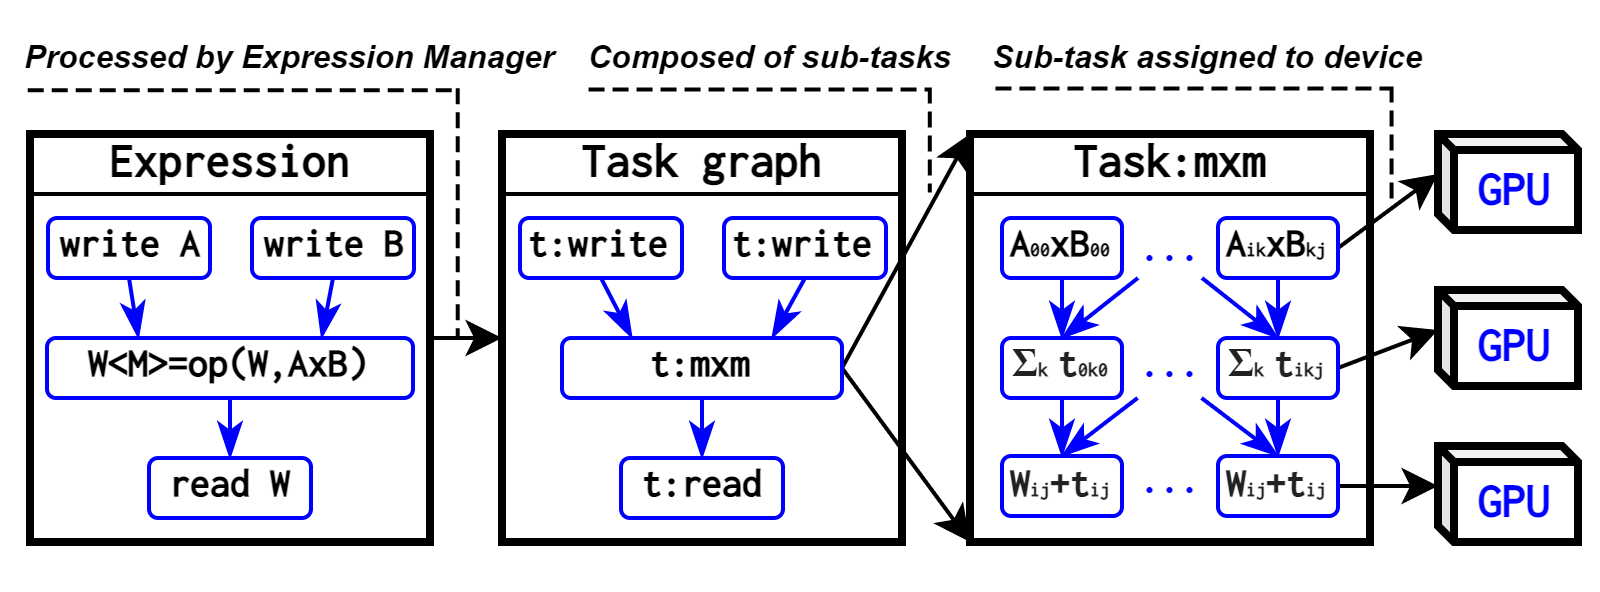
\includegraphics[width=0.99\linewidth]{figures/library_architecture.png}
\caption{Library expression processing architecture.}
\label{fig:architecture}
\end{figure}
    
\subsection{Matrices and Vectors}

Library provides general \textit{M-by-N Matrix} and \textit{N Vector} primitives.
Underlying primitives types is specified by \textit{Type} object. 
Internally primitives are stored in a hybrid storage in a form of two- or one- dimensional blocks' grid respectively. 
Each block is empty (not stored) or store some data in any format. Blocks are immutable, they can be safely shared across computational devices.

Currently only COO blocks are supported. Format choice is motivated by its simplicity and easy of implementation. 
Other formats, such as CSR, CSC, DCSR, Dense, etc. can be added to the library by either implementation of formats convertation or by the specialization of \textit{Algorithm} for concrete format.

\subsection{Algebraic Operations}

Library supports all commonly used linear algebra operations, such as \textit{mxm}, \textit{vxm}, \textit{eadd}, \textit{reduce}, \textit{transpose}. 
More operations coming later, since library still in development.
Interface of operations is designed in similar fashion as GraphBLAS ones. 
It supports \textit{masking}, \textit{accum} of the result, \textit{add} and/or \textit{mult} user-functions specification, and \textit{descriptor} object for additional operation tweaking.

\subsection{Implementation Details}

Library uses OpenCL 1.2 API as underlying compute API. 
Boost Compute~\cite{10.1145/2909437.2909454:boost:compute} is utilized as a high-level library on top of the OpenCL functionality. 
It provides thread-safe kernel caching, meta-kernel programming, and a set of basic parallel primitives such as \textit{device vector}, \textit{sort}, \textit{reduce}, \textit{scan}, etc. which was extended further to meet this project requirements.
Taskflow~\cite{Huang2022TaskflowAL} is used as tasking library. It supports task-dependencies and dynamic tasking, utilized in order to create and execute sub-tasks. 

User-defined \textit{Types} are represented as POD-structures, and handled by the library as a fixed-size sequences of bytes.
User-defined \textit{Functions} are effectively textual strings with OpenCL code, injected into generalized meta-kernels.
Library has a number of predefined types, such as \textit{signed/unsigned integers}, \textit{floating point} types, and a set of common operations, such as \textit{arithmetic}, \textit{logic}, \textit{first/second}, etc.

For particular blocked \textit{vxm} and \textit{mxm} \textit{Algorithms} implementations ESC algorithm~\cite{10.1145/2699470:esc:algo} for COO blocks is employed. 
Element-wise addition and masking are based on tiled GPU Merge Path~\cite{inproceedings:gpu_merge_path} algorithm. 
The code is generalized and is written in a form of meta-kernels, so actual functions for elements reduction or multiplication are injected later.
Kernel compilation is done on demand if no previously cached entry present.


\section{Evaluation}

For performance analysis of proposed solution we evaluated some most common graph algorithms using real-world sparse matrix data. 
As a baseline for comparison we chose LAGraph~\cite{szarnyas2021lagraph} in connection with SuiteSparse~\cite{10.1145/3322125} as a CPU tool, Gunrock~\cite{7967137} and GraphBLAST~\cite{yang2019graphblast} as a Nvidia GPU tools. 
Also, we tested algorithms on several devices with distinct OpenCL vendors in order to validate portability of the proposed solution. 
In general, these evaluation intentions are summarized in the following research questions. 

\vspace{0.2cm}
\begin{itemize}
    \item[\textbf{RQ1}] What is the performance of the proposed solution relative to existing tools for both CPU and GPU analysis?
    
    \item[\textbf{RQ2}] What is the portability of the proposed solution with respect to various device vendors and OpenCL runtimes?
\end{itemize}

\subsection{Evaluation Setup}

For evaluation, we use a PC with Ubuntu 20.04 installed, which has 3.40Hz Intel Core i7-6700 4-core CPU, DDR4 64Gb RAM, and Nvidia GeForce GTX 1070 GPU with 8Gb VRAM. 
Host programs were compiled with GCC 9.3.0 compiler. Programs using CUDA were compiled with GCC 8.4.0 and Nvidia NVCC 10.1.243 compiler.
Release mode and maximum optimization level was enabled for all tested programs. 
Data loading time, preparation, format transformations and host-device initial communications are excluded from time measurements. 
All tests are averaged across 10 runs.
Additional warm-up run for each test execution is excluded from measurements.

\subsection{Graph Algorithms}

For preliminary study \textit{breadth-first search} (bfs) and \textit{triangles counting} (tc) algorithms were chosen, since they allows analyse the performance of \textit{vxm} and \textit{mxm} operations, rely heavily on \textit{masking}, and utilize \textit{reduction} or \textit{assignment}. 
BFS implementation utilizes automated vector storage from sparse to dense switch and only \textit{}{push optimization}. 
TC implementation uses masked \textit{mxm} of source lower-triangular matrix with second transposed argument.

\subsection{Dataset}

Nine graph matrices were selected from the Sparse Matrix Collection at University of Florida~\cite{dataset:10.1145/2049662.2049663}. 
Information about graphs is summarized in Table~\ref{dataset:info}. 
All datasets are converted to undirected graphs. 
Self-loops and duplicated edges are removed.

\begin{table}[htbp]
\caption{Dataset description.} 
\begin{center}
    \rowcolors{2}{black!2}{black!10}
    \begin{tabular}{|l|r|r|r|}
    \hline
    Dataset & Vertices  & Edges & Max Degree \\
    \hline
    \hline
    coAuthorsCiteseer & 227.3K &   1.6M &    1372 \\
    coPapersDBLP      & 540.4K &  30.4M &    3299 \\
    hollywood-2009    &   1.1M & 113.8M &  11,467 \\
    roadNet-CA        &   1.9M &   5.5M &      12 \\
    com-Orkut         &     3M &   234M &   33313 \\
    cit-Patents       &   3.7M &  16.5M &     793 \\
    rgg\_n\_2\_22\_s0 &   4.1M &  60.7M &      36 \\
    soc-LiveJournal   &   4.8M &  68.9M &  20,333 \\
    indochina-2004    &   7.5M & 194.1M & 256,425 \\
    \hline
    \end{tabular}
    \label{dataset:info}
\end{center}
\end{table}

\subsection{Results}

Table~\ref{results} presents results of the evaluation and compares performance of Spla against other tool on different execution platforms.
Tools are grouped by the type of the device for the execution, where either Nvidia GPU or Intel CPU are used. 
Cell left empty if tested tool failed to analyse graph due to \textit{out of memory} exception.

In general, Spla BFS shows acceptable performance, especially on graphs with large vertex degree, such as soc-LiveJournal and com-Orkut.
On graphs roadNet-CA and rgg it has a significant performance drop due to the nature of underlying algorithms and data structures. 
Firstly, library utilizes immutable data buffers. Thus, iteratively updated dense vector of reached vertices must be copied for each modification, what dominates the performance of the library on a graph with large search depth. 
Secondly, Spla BFS does not utilise \textit{pull optimization}, what is critical in a graph with relatively small search frontier. 

Spla TC has a good performance on GPU, which is better in all cases that reference SuiteSparse solution. 
But in most tests GPU competitors, especially Gunrock, show smaller processing times. 
GraphBLAST shows better performance as well. 
Library utilises masked SpGEMM algorithm, the same as in GraphBLAST, but without \textit{identity} element to fill gaps. 
Library explicitly stores all non-zero elements, and uses mask to reduce only non-zero while evaluating dot products of rows and columns. 
What causes extra divergence inside work groups. 
On Intel device Spla shows better performance compared to SuiteSparse on com-Orkut, cit-Patents and soc-LiveJournal. 
A possible reason is the large lengths of processed rows and columns in the product of matrices.

Gunrock shows nearly best average performance due to its specialized and optimized algorithms.
Also, it has good time characteristics on a mentioned earlier roadNet-CA and rgg in BFS algortihm. 
GraphBLAST follows Gunrock and show good performance as well. 
But it runs out of memory on a two significantly large graphs con-Orkut and indochina-2004. 
Spla does not rut out of memory on any test due to simplified storage scheme.

\begin{table}[htbp]
\caption{Graph algorithms evaluation results.\\Time in milliseconds (lower is better).} 
\begin{center}
    \begin{tabular}{|l|r|r|r|r|r|}
    \hline
    \multirow{2}{*}{Dataset} & \multicolumn{3}{c|}{Nvidia} & \multicolumn{2}{c|}{Intel} \\
    \cline{2-6}
    & GR & GB & SP & SS & SP \\
    \hline
    \hline
    \multicolumn{6}{|c|}{BFS} \\
    \hline
    \rowcolor{black!10} hollywood-2009    &  20.3 &  82.3 &   36.9 &   23.7 &   303.4 \\
    \rowcolor{black!2 } roadNet-CA        &  33.4 & 130.8 & 1456.4 &  168.2 &   965.6 \\
    \rowcolor{black!10} soc-LiveJournal   &  60.9 &  80.6 &   90.6 &   75.2 &  1206.3 \\
    \rowcolor{black!2 } rgg\_n\_2\_22\_s0 &  98.7 & 414.9 & 4504.3 & 1215.7 & 15630.1 \\
    \rowcolor{black!10} com-Orkut         & 205.2 & -- -- &  117.9 &   43.2 &   903.6 \\
    \rowcolor{black!2 } indochina-2004    &  32.7 & -- -- &  199.6 &  227.1 &  2704.6 \\
    \hline
    \hline
    \multicolumn{6}{|c|}{TC} \\
    \hline
    \rowcolor{black!10} coAuthorsCiteseer &   2.1 &    2.0 &    9.5 &    17.5 &    64.9 \\
    \rowcolor{black!2 } coPapersDBLP      &   5.7 &   94.4 &  201.9 &   543.1 &  1537.8 \\
    \rowcolor{black!10} roadNet-CA        &  34.3 &    5.8 &   16.1 &    47.1 &   357.6 \\
    \rowcolor{black!2 } com-Orkut         & 218.1 & 1583.8 & 2407.4 & 23731.4 & 15049.5 \\
    \rowcolor{black!10} cit-Patents       &  49.7 &   52.9 &   90.6 &   698.3 &   684.1 \\
    \rowcolor{black!2 } soc-LiveJournal   &  69.1 &  449.6 &  673.9 &  4002.6 &  3823.9 \\
    \hline
    \hline
    \multicolumn{6}{l}{Tools: Gunrock (GR), GraphBLAST (GB), SuiteSparse (SS), Spla (SP).} \\
    \end{tabular}
    \label{results}
\end{center}
\end{table}
 
% Two GPU

% \begin{table}[htbp]
%     \caption{Table Type Styles}
%     \begin{center}
%     \begin{tabular}{|c|c|c|c|}
%     \hline
%     \textbf{Table}&\multicolumn{3}{|c|}{\textbf{Table Column Head}} \\
%     \cline{2-4} 
%     \textbf{Head} & \textbf{\textit{Table column subhead}}& \textbf{\textit{Subhead}}& \textbf{\textit{Subhead}} \\
%     \hline
%     copy& More table copy$^{\mathrm{a}}$& &  \\
%     \hline
%     \multicolumn{4}{l}{$^{\mathrm{a}}$Sample of a Table footnote.}
%     \end{tabular}
%     \label{tab2}
%     \end{center}
% \end{table}

\section{Conclusion}

In this paper we present a library for sparse Boolean linear algebra which implements such basic operations as matrix-matrix multiplication and element-wise matrix-matrix addition in both Cuda and OpenCL.
Evaluation shows that our Boolean-specific implementations faster and require less memory than generic, not the Boolean optimized, operations from state-of-the-art libraries. 
Thus, the specialization of operations for this data type makes sense. 

The first direction of the future work is to integrate all parts (OpenCL and Cuda backends) into a single library and improve its documentation and prepare to publish.
Moreover, it is necessary to extend the library with other operations, including matrix-vector operations, masking, and so on.
As a result a Python package should be published.

Another important step is to evaluate the library on different algorithms and devices.
Namely, algorithms for RPQ and CFPQ should be implemented and evaluated on related data sets.
Also, it is necessary to evaluate OpenCL version on FPGA which may require additional technical effort and code changes.

Finally, we plan to discuss with GraphBLAS community possible ways to use our library as a backend for GraphBLAST or SuiteSparse in case of Boolean computations.
Moreover, it may be possible to use implemented algorithms as a foundation for generalization to arbitrary semirings.


%%
%% The acknowledgments section is defined using the "acks" environment
%% (and NOT an unnumbered section). This ensures the proper
%% identification of the section in the article metadata, and the
%% consistent spelling of the heading.
\begin{acks}
The research was supported by the Russian Science Foundation,
grant №18-11-00100.

We thank Adrian Johnstone for his pointing out the Generilized LL algorithm in our discussion at Parsing@SLE--2013 which gave us the motivation to develop the presented solution.

%We thank  George Fletcher for his discussion of evaluation of different CFPQ algorithms for Neo4j.

%We thank Tobias Lindaaker, 

\end{acks}

%%
%% The next two lines define the bibliography style to be used, and
%% the bibliography file.
\bibliographystyle{ACM-Reference-Format}
\bibliography{gll4graph}

%%
%% If your work has an appendix, this is the place to put it.
%\appendix

%\section{Research Methods}

\end{document}
\endinput
%%
%% End of file `sample-sigconf.tex'.
